\documentclass[]{tufte-handout}
\usepackage{amsmath,amssymb,amsthm,color}
\usepackage[pdftex]{graphicx}

 
\title{COMP 161 - Lecture Notes - 02 - Shells, part 1}
\date{Spring 2014}

\begin{document}
\maketitle

\begin{abstract}
Shotts' tutorial introduces the shell\sidenote{\url{http://linuxcommand.org/lc3_lts0010.php}} but discusses how to access it as if you're accessing the shell of the computer in front of you.  In this class, we'll be accessing the shell of a the departmental server on the second floor of the CSB.  So, we'll need to figure out how to access the shell of that computer remotely using a Secure Shell\sidenote{SSH} client. We'll also briefly discuss some common patterns in shell commands, the command to that you'll use to submit most of your assignments, and how to move files to and from the remote system. 
\end{abstract}

\section{The Shell}

As Shotts explains quite well, the \textit{shell} is your command line interface with the Operating system\sidenote{which is the interface to the hardware}.  We're using \textit{bash}\sidenote{run the command \textit{echo \$SHELL} to see which shell you're running}, but there are many other shells you could check out\sidenote{ksh,tcsh, and zsh}.  These shells are all available for any Linux or Mac OS-X based system. If you want to explore a similar shell system for Windows, then you can check out Microsoft's PowerShell\sidenote{\url{http://msdn.microsoft.com/en-us/library/dd835506(v=vs.85).aspx}}.    

The real power of shells comes from the fact that they are \textit{programming languages}\sidenote{or scripting languages}.  More specifically, they are languages designed to let you write programs involving the activities carried out with the shell\sidenote{typically called \textit{scripts}}.  This means that using you shell language, you can likely automate most of the repetitive tasks you carry out on a regular basis.  For example, I used a bash script I wrote in order to create all of your accounts, generate random initial passwords for them, and be sure other account related settings were where they needed to be.  Without this script I would have needed to type something like five commands per account. For a class of $n$ students that $5n$ commands.  So, even for modest sized classes, that script saves me from a lot of repetitive typing. Perhaps more importantly, it prevents me from making typos and inadvertently messing something up\sidenote{The value of this is huge. We all make mistakes.}. 

We're not going to get into shell scripts, but Shotts has a wonderful tutorial on them\sidenote{\url{http://linuxcommand.org/lc3_writing_shell_scripts.php}}. I highly recommend you check it out.  If that leaves you wanting more, there are an insane number of \textit{bash scripting} tutorials out there\sidenote{Look around \url{http://tldp.org} for starters}.

\section{Secure, Remote Access} 

It is very common to need or want remote access to the shell of a computer you're not currently sitting in front of. Smart users want to do so in a way that ensures nobody can easily snoop on what they're doing. Thus, a \textit{secure shell} is needed. The defacto way to accomplish secure remote access to the shell is through an SSH client-server setup\sidenote{\url{http://www.openssh.com/}}.  The computer to which you want access\sidenote{the server} must be running an SSH server program, and the computer with which you're connecting\sidenote{the client} needs an SSH client program.  

If your client is running Linux or OS X, then you're in luck. You already have an ssh client available through your terminal.  If you're running Windows\sidenote{like all our computer labs do}, then you need to get a client. Thankfully, there is a wonderful, free SSH client for Windows called PuTTy\sidenote{\url{http://www.chiark.greenend.org.uk/~sgtatham/putty/download.html}}.  The PuTTy ssh client is available on all campus computers\sidenote{W:$\backslash$Apps$\backslash$mathcs$\backslash$putty$\backslash$PUTTY.EXE. I'd make a shortcut to it on your desktop if I were you.}. 

I'll break down the process of logging in to a computer's shell with SSH using a CLI client and PuTTy.  First, I want to point a few thing you'll experience the first time you log in so that you'll be ready for them. Once you know what's different the first time, we'll talk about what's going to happen the rest of the time.

\subsection{The first time you login}

A few things out of the ordinary happen the first time you login.  
\begin{itemize}
\item The first time a client and server communicate, they must establish trust.
\item On our servers, the first time you've ever used the account, you'll need to reset your password to a password that only you know. \end{itemize}

A big part of security is trust. So the first time an ssh client logins to an ssh server it must establish trust.  This means your client will ask you if you know the server that you're logging in to and if it should really connect to that server. A server is identified not by it's name or address but by a unique \textit{key}\sidenote{very big number}. So, your job is to tell your client that connections to the server with that key are trusted.  Here's what that looks like in linux:

\vspace{.1in}
\begin{center}
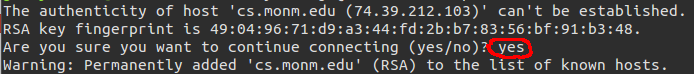
\includegraphics[scale=.5]{linux-knownhost.png}
\end{center}
\vspace{.1in}


and in Windows with PuTTy.

\vspace{.1in}
\begin{center}
\textbf{ADD IMAGE}
\end{center}
\vspace{.1in}

There's really \textbf{no reason anyone other than you should know your password}\sidenote{including system administrators like me}.  The account begins with a randomly generated password\sidenote{given to you in class}.  The first time you login to your account, you'll be forced to reset your password. There are two big things to note about this process:
\begin{enumerate}
\item When you're typing a password, \textit{it looks like nothing is happening on the screen}\sidenote{this is always true and always weirds at least a few students out}
\item When you're done, you'll be booted from the server and will have to log back in with the new password.
\end{enumerate}
The process is straight forward if you \textit{read and follow the directions}\sidenote{at lease a few people don't read the prompts and mess up their password. It's fixable, but easily avoidable by \textbf{reading the directions}}.

\subsection{Linux and OS X}

Linux and OS X both come with a command-line SSH client installed.  In order to access it you need to first launch your local \textit{terminal}\sidenote{this is the shell access Shotts talks about}. Once your local terminal is up and running the command is fairly straight forward. The most basic command dictates the port\sidenote{-p 22}, username, and server\sidenote{cs.monm.edu} to which you're connecting. The complete command looks like: \textit{ssh -p 22 user@server}.  Here you see an example of me logging in from my Linux machine.

\vspace{.1in}
\begin{center}
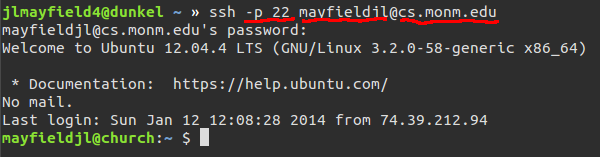
\includegraphics[scale=.5]{linux-sshlogin.png}
\end{center}
\vspace{.1in}

As you can see, once you enter the command, you'll connect to the server and be asked for the password for the given username. Once you're done with your shell session, use the command \textit{exit} to logout. 

\subsection{PuTTy (Windows)}

PuTTy is  GUI based SSH client.  On the surface it is very easy to get logged in, but it does have one little quirk you'll want to deal with. By default, PuTTy reads the letters coming from the server using a European standard.  The result is that some of the letters get garbled\sidenote{you'll probably see it first when you run the compiler for C++}. So, to fix this we need to tell PuTTy to use UTF-8, the standard used by the server.  You can either set this every time you launch PuTTy\sidenote{and waste a minute} or set it once and save your PuTTy settings. I'll show you how to do the later, and get logged in.  

To set the encoding to UTF-8 you need to navigate the settings to \textit{Window$>$Translation} and select \textit{UTF-8} as the Remove character set.

\vspace{.1in}
\begin{center}
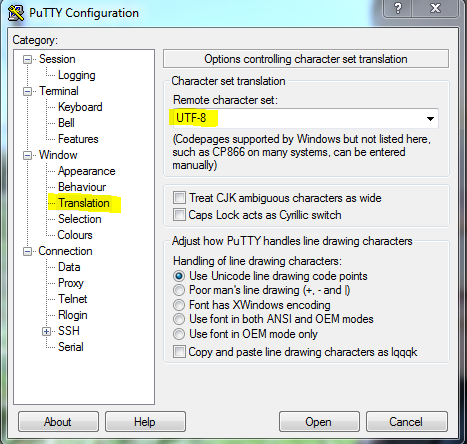
\includegraphics[scale=.75]{Putty-SetUTF8.PNG}
\end{center}
\vspace{.1in}

Once you've done that, navigate back to the session options, fill in the \textit{Host Name} and \textit{Port}, and then fill in a Saved Sessions name. With all of that filled in, you can hit save to save the encoding and session info for future use.

\vspace{.1in}
\begin{center}
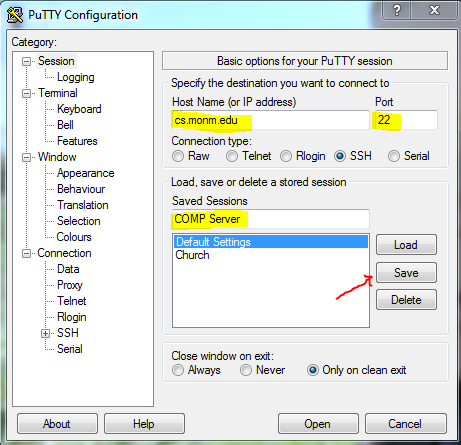
\includegraphics[scale=.75]{Putty-SaveSettings.PNG}
\end{center}
\vspace{.1in}

With the right encoding and server information saved, you can now load your settings and open the connection\sidenote{this is what you should be doing all but the first login. unless you like to waste a minute per login with a tasks that are easily automated...}. Highlight the saved session name, hit \textit{Load}, then hit \textit{Open}. 

\vspace{.1in}
\begin{center}
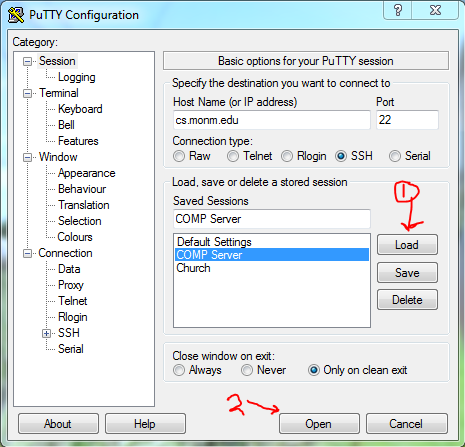
\includegraphics[scale=.75]{Putty-LoadAndOpen.PNG}
\end{center}
\vspace{.1in}

You'll now be prompted for your username and password. 

\vspace{.1in}
\begin{center}
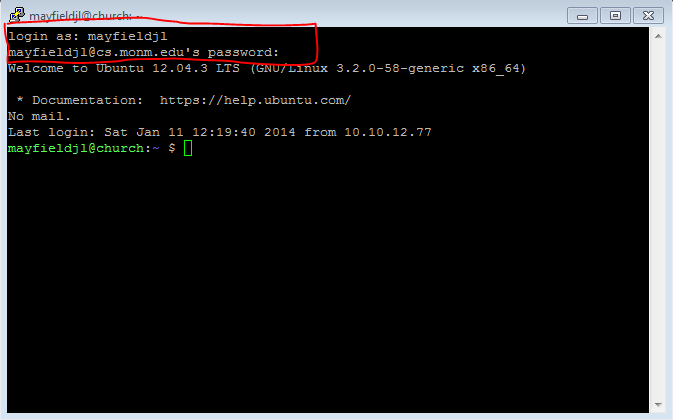
\includegraphics[scale=.75]{Putty-Login.PNG}
\end{center}
\vspace{.1in}

When you're all done with the shell, the command \textit{exit} will log you out of the server.  


\section{Submitting assignments with \textit{handin}}

A script written for us by a former CS professor\sidenote{Thanks, Don Blaheta!} here at Monmouth allows you to submit most of your assignments via the server. The name of the script\sidenote{and the command} is \textit{handin}.  You'll work out its usage in the first lab.  If you need a refresher, the following command will give you the help text for the command.

\begin{verbatim}
handin -h
\end{verbatim}

\section{Moving files}

Because of \textit{handin}, you'll never really need to move files to and from the server.  However, students regularly want to do this so I'll discuss a few ways to do this here.  The traditional method is to piggy back on the SSH connection using \textit{secure file transfer protocol}\sidenote{sftp}. However, I personally use the cloud storage service Dropbox\sidenote{\url{http://dropbox.com}} which has a command-line client. 

\subsection{sftp and psftp}

If a computer is running an SSH server, then chances are it can handle sftp connections as well.  An sftp client runs its own little CLI, so once you're logged in, there's a series of commands you'll use to move files. Many of them are the same as the shell commands you're learning, but this time there's a version for your local machine and another for the server\sidenote{run the command \textit{help} from within an sftp session to see the full list of commands}.


In Linux and OS X, there is a command-line client that you launch in pretty much the same way as ssh: \textit{sftp user@server}. 

\vspace{.1in}
\begin{center}
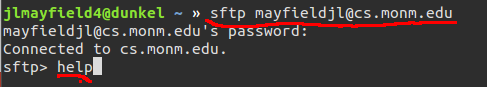
\includegraphics[scale=.5]{linux-sftplogin.png}
\end{center}
\vspace{.1in}

In Windows, you can use the PuTTy SFTP\sidenote{psftp} client, which can be downloaded\sidenote{and found on the campus network} from the sample place you got PuTTy. Just launch \textit{psftp.exe} and then follow the prompts to log on to the server. 

\vspace{.1in}
\begin{center}
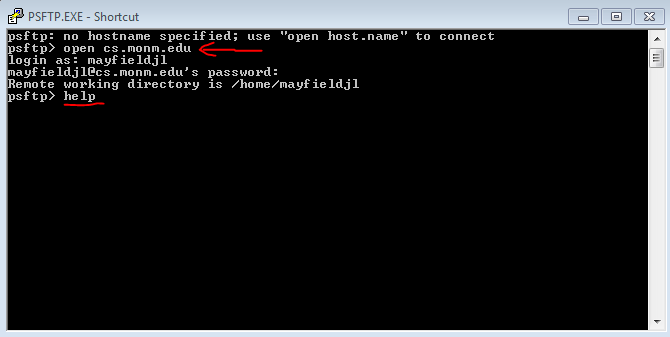
\includegraphics[scale=.75]{PSFTP-loginAndHelp.PNG}
\end{center}
\vspace{.1in}

Once you're logged in, it runs the same as the Linux client. Once again, use the \textit{help} command to see the list of sftp commands.

\subsection{Dropbox}

I'm a big Dropbox fan\sidenote{not a paid spokesperson}. With a minimal amount of effort, it lets me share files between my personal computer, my work computer, the servers I use at work, and my smartphone.  Those same file are also accessible via the web if I can't get to one of those devices.

If you want to go the dropbox route you'll need a dropbox account. If you need or want a dropbox account and want to do your professor a solid, signup via this link\sidenote{I get free extra storage if you do}:
\begin{quote}
\url{https://db.tt/XOjdfkS}
\end{quote}
If you don't want me to get free storage with them, then feel free to sign-up from their website\sidenote{\url{http://dropbox.com}}. 

Once you have an account you need to install the Linux Command-Line client on the server.  
\begin{enumerate}
\item Login to the server
\item Follow these \textit{Install Dropbox via the command line} instructions: \url{https://www.dropbox.com/install?os=lnx}
\begin{itemize}
\item Alternatively: \url{http://www.dropboxwiki.com/tips-and-tricks/install-dropbox-in-an-entirely-text-based-linux-environment}
\end{itemize}
\item Then look at these instructions on using the client: \url{http://www.dropboxwiki.com/tips-and-tricks/using-the-official-dropbox-command-line-interface-cli}
\end{enumerate}

Once you're up and running, it's pretty much like having a folder that when you put files and folders in it, will sync them up with your dropbox.  There are a few things to keep in mind with Dropbox:
\begin{itemize}
\item You need to restart it every time the server reboots\sidenote{bound to happen a few times a semester}
\item You should not work out of your dropbox folder\sidenote{It's a dropbox, not a workspace}. It'll probably get your in trouble.
\end{itemize}

\end{document}
